\documentclass[a4paper,12pt]{report}

\usepackage[utf8]{inputenc} % vagy latin2 helyett utf8
\usepackage[T1]{fontenc}      % karakterkódolás
\usepackage[magyar]{babel}    % magyar beállítások
\frenchspacing                % helyközök
%\usepackage{times}           % betûtípus
\usepackage{lmodern}          %   vagy inkább ez

\usepackage[margin=2.5cm,left=3.5cm,includeheadfoot]{geometry}
                              % margók
\usepackage{graphicx}         % képekhez
\usepackage{setspace}         % sorköz
\onehalfspacing               % másfeles

% from: http://stackoverflow.com/questions/741985/latex-source-code-listing-like-in-professional-books?rq=1
\usepackage{epstopdf}
\usepackage{listings}
\usepackage{courier}
\usepackage{caption}

\usepackage{sidecap}

\usepackage{color}
\definecolor{deepblue}{rgb}{0,0,0.5}
\definecolor{deepred}{rgb}{0.6,0,0}
\definecolor{deepgreen}{rgb}{0,0.5,0}

\usepackage{graphics}
 \lstset{
         basicstyle=\footnotesize\ttfamily, 
         %numbers=left,              
         numberstyle=\tiny,          
         numbersep=5pt,              
         tabsize=3, 
         language=Python,
         otherkeywords={Walk, begin, end, endif, true, false, Operators, Keywords, elsif },
         extendedchars=true,         
         breaklines=true,       
         emph={Walk,Resolve,PROGRAM, STATEMENT, ASSIGN_STATEMENT, IF_STATEMENT, WHILE_STATEMENT,
                        FUNCALL_STATEMENT, EXPRESSION, FUNCALL_EXPRESSION, ARRAY_ACCESSOR, FIELD_ACCESSOR},          % Custom highlighting
         emphstyle=\ttb\color{deepred},    % Custom highlighting style
         %keywordstyle=\color{red},
         keywordstyle=\ttb\color{deepblue},
        	frame=b,         
        %keywordstyle=[1]\textbf,    
         stringstyle=\color{deepgreen}\ttfamily, 
         %stringstyle=\color{deepgreen},
         showspaces=false,           
         showtabs=false,             
         xleftmargin=17pt,
         framexleftmargin=17pt,
         framexrightmargin=5pt,
         framexbottommargin=4pt,
         %backgroundcolor=\color{lightgray},
         showstringspaces=false          
 }
 \lstloadlanguages{% Check Dokumentation for further languages ...
         Python
 }
    %\DeclareCaptionFont{blue}{\color{blue}} 

  %\captionsetup[lstlisting]{singlelinecheck=false, labelfont={blue}, textfont={blue}}
  \usepackage{caption}
  \usepackage{hyperref}
\DeclareCaptionFont{white}{\color{white}}
\DeclareCaptionFormat{listing}{\colorbox[cmyk]{0.43, 0.35, 0.35,0.01}{\parbox{\textwidth}{\hspace{15pt}#1#2#3}}}
\captionsetup[lstlisting]{format=listing,labelfont=white,textfont=white, singlelinecheck=false, margin=0pt, font={bf,footnotesize}}




\begin{document}

\renewcommand\lstlistingname{Algoritmus}
\renewcommand\lstlistlistingname{Algoritmusok}

% ------------------------------------------------------------------------------
% Címlap

\begin{titlepage}

\noindent
\parbox[m]{0.2\textwidth}{
%
\includegraphics[width=0.2\textwidth]{elte_cimer_ff.eps}     % fekete-fehér
 
\includegraphics[width=0.2\textwidth]{elte_cimer_szines.eps} % színes
}
\hfill
\parbox[m]{0.7\textwidth}{
\begin{center}
\begin{large}
\textsc{
Eötvös Loránd Tudományegyetem\\
\vspace{0.5pc}
Informatikai Kar\\
\vspace{0.5pc}
Programozáselmélet és Szoftvertechnológiai Tanszék\\
}
\end{large}
\end{center}
}

\vspace{1pc}
\hrule

\vfill

\begin{center}
{\LARGE Térinformatikai szkriptnyelv megvalósítása}
\end{center}

\vfill

\noindent
\hspace*{0.05\textwidth}
\parbox{0.45\textwidth}{
{\it Témavezetõ:}
\bigskip

{\Large Giachetta Roberto}
\smallskip

tanársegéd
}
\hfill
\parbox{0.45\textwidth}{
{\it Készítette:}
\bigskip

{\Large Marczinus Dávid}
\smallskip

programtervezõ informatikus BSc
}


\vfill

\begin{center}
{\large {\it Budapest, 2013}}
\end{center}

\end{titlepage}


% ------------------------------------------------------------------------------
% Témabejelentõ

\vspace*{\fill}
\begin{center}
Ehelyett az oldal helyett a Szakdolgozat-téma bejelentõ szerepel.
\end{center}
\vfill
\thispagestyle{empty}
\newpage
\setcounter{page}{1}

% ------------------------------------------------------------------------------
% Tartalomjegyzék

\tableofcontents

% ------------------------------------------------------------------------------


\chapter{Bevezetõ}

A modern szoftverfejlesztésben kiemelt szerepet kapnak a rendkívül robosztus, fordított nyelvek, mint a C\#, a Java vagy a C++. Az utóbbi évek azonban új trendeket hoztak magukkal: többé nem lehet interpretált programozási nyelvek kapcsán azt hallani, hogy azok "csak" szkriptnyelvek. Az internetet dominálják a különböző JavaScriptben írt keretrendszerek. Az webfejlesztés új sztenderdjét jelenti a Ruby on Rails, illetve a Pythonban íródott Django framework. Egyre több asztali alkalmazást írnak szkriptnyelvekben, amik ráadásul nagyrészt platform-függetlenek. Bár a fordított nyelvek fontossága vitathatatlan, az utóbbi évek alapján úgy tűnik, hogy az interpretált nyelveké a jövő. \\

Mi az oka ennek? Valószínűleg a legnyomósabb érv a szkriptnyelvek mellett a rendkívül gyors fejlesztési ütem. Elképesztően gyorsan lehet például Ruby on Railsben jól működő webes alkalmazásokat írni, ráadásul a jól megírt Ruby kódot öröm olvasni, nem is beszélve az RSpec-ben megírt egységtesztekről. \\
A gyors fejlesztés mellett érdemes azt is figyelembe venni, hogy modern környezetben gyakran teljesen jelentéktelen a sebességveszteség ami egy szkriptnyelv használatával jár. \\
Természetesen az sem elhanyagolható, hogy ezeknek a nyelveknek a szintaxisa ( és a szemantikája ) lényegesen gyorsabban tanulható, mint példának okán a C++-é. Emellett a szkriptnyelvek többsége metaprogramozásra is ad lehetőséget, amivel a nyelv szakértői saját izlésük szerint akár át is szabhatják a nyelvet.
\\

Az általános trendeken túl az is észrevehető, hogy egyre több cég és egyre több projekt alkalmaz úgynevezett DSL-eket (Domain Specific Language\cite{dsl}) különböző célokra. Dolgozatom során én is egy ilyen domain-specifikus nyelv implementálásával foglalkoztam az AEGIS keretrendszeren belül. Ennek a nyelvnek a legfőbb célja, azon túl, hogy természetesen minden általános vezérlési szerkezetet támogat, az, hogy az AEGIS-ben definiált osztályokat és azok eljárásait interpretálva, batch szkriptként tudjuk futtatni.  \\
Mivel a dolgozat az AEGIS keretrendszerhez készült, így a felhasználandó technológiák adottak voltak: C\# és .NET. Ezen felül magát a nyelvet ANTLR\cite{antlr} v3.5-ben valósítottam meg. \\ 

% referencia AEGIS-hez és ANTLR-hez
A nyelv implementálásán túl terveztem egy grafikus felületet, amivel kapcsolatban szigorú elvásáraim voltak. Az első az volt, hogy a felületnek modernnek és intuitívnek kell lennie. A második a reszponzivitás volt, azaz különösen fontosnak tartottam, hogy a kódszerkesztő gyors legyen, a program használható legyen akkor is, ha éppen forráskód interpretálása folyik, illetve a futtatás bármikor megszakítható legyen, akár végtelen ciklusba kerülve is. \\


% ------------------------------------------------------------------------------

\chapter{Projektdefiníció}
\section{Elméleti háttér}
\subsection{Interpreterek}

%------------

\subsubsection{Bytecode interpreterek}
Megvalósításukat tekintve az összes szkriptnyelvet be tudjuk sorolni két nagyon eltérő kategóriába. Az első ezek közül a bytecode interpreterek halmaza. Ezek a forráskód alapján egy köztes formát, bytecode-ot hoznak létre, amiket később egy virtuális gép futtat le. Rengeteg vonzó tulajdonságuk van, köztük a kiváló sebesség, éppen ezért az összes ismert és népszerű szkriptnyelv, köztük a Python és a Ruby, bytecode interpretálást használ. A tervezési fázisban még úgy gondoltam, hogy az általam megvalósított nyelv is ilyen lesz, hiszen a .NET virtuális gépe adott volt, illetve a .NET Reflection könyvtárán keresztül a lehetőség lett volna közvetlen bytecode generálásra is. Azonban az hamar kiderült, hogy a legegyszerűbb konstrukciók bytecode-dá történő fordítása is rendkívül körülményes, éppen ezért az interpreterek megvalósításának a másik módját választottam.

%------------ Bytecode interpreterek

\subsubsection{AST interpreterek}

Az AST (\textit{Abstract Syntax Tree}) interpreterek megvalósításukat tekintve lényegesen intuitívabbak, mint a bytecode interpreterek. Lényegében egy külső eszközben leírjuk a nyelv specifikációját, majd ezen eszköz a neki adott forráskódokból előbb parse tree-t, majd abból AST-t hoz létre, amit pedig már az adott nyelvi környezetben kell feldolgozni és értelmezni.\\
% itt egy ábra parse tree és AST összehasonlításáról
Bár az AST interpreterek viszonylag intuitívak, az absztrakt szintaxisfák feldolgozásáról az irodalom nagyon szűkös. Az egyetlen használható forrás az AEGIScript megvalósítása során \textit{Terence Parr: Language Implementation Patterns}\cite{lip} című könyvve volt, azonban ez is csak a szimbólumtáblák és a scope-ok implementálásában tudott segíteni. Az AST-k feldolgozására ezért saját algoritmusokat kellett kidolgoznom, amikkel szemben fontos elvárás volt, hogy később könnyen bővíthetőek legyenek új nyelvi elemekkel, éppen ezért általános esetre tökéletesen kellett működniük.

%------------ AST interpreterek

\section{Absztrakt szintaxisfa bejárások}
Algoritmizálás szempontjából egy absztrakt szintaxisfa összesen két nagyon különböző csúcsot különböztet meg: az egyik az utasítás (\textit{statement}), a másik pedig a kifejezés (\textit{expression}).
\\
Utasítások építik fel alapvetően a programot, ezek tesznek ki egy teljes sort a programkódban. Visszatérési értékük nincs a nyelvek nagy részében, bár egyes nyelvek, mint az Erlang ezekhez is rendelnek értéket.
\\
Kifejezések értelemszerűen valamilyen visszatérési értékkel rendelkező kódrészletek, mint például aritmetikai kifejezések, függvényhívások vagy változó hozzáférések. Ezek nyelvtani szabályok szerint tetszőleges mélységig egymásba ágyazhatóak.
\\
Mivel a két csúcstípus egyértelmű különbségekkel rendelkezik, már a tervezési fázisban is két külön algoritmust írtam az értelmezésükre. Mindkét algoritmusban közös, hogy mélyen rekurzívak, ezzel biztosítva azt, hogy tetszőleges mélységig ágyazhassunk egymásba utasításokat és kifejezések. Emellett még közös tulajdonságuk, hogy "double dispatching"-et használnak, azaz kihasználják, hogy a csúcsok közös őstől származnak, és futási idejű típusuknak megfelelően kerülnek a megfelelő függvényhez feldolgozásra.

%----------------------------- 

\subsection{Utasítások bejárása}
Az utasítások feldolgozására írt algoritmus Walk-nak neveztem el, mivel egyszerűen végigjárja a különböző utasítás-csúcsokat, de konkrétan nem manipulálja őket. Minden egyes vezérlési struktúrához definiáltam egy Walk függvényt, ami megfelően kezeli az adott szerkezetet. Emellett, külső interfésznek egy olyan absztrakciós szintet írtam szintén Walk néven, ami könnyen bővíthető a jövőben újabb szerkezetekkel.

%------------ 

\subsubsection{Kezdőcsúcs bejárása}
A kezdőcsúcs típusát BeginNode-ként definiáltam. Ezen csúcs gyerekei a program legfelsőbb szintű utasításai, és ezen utasítások definiálják a program globalscope-ját. \\
Bejárási logikája triviális, egyszerűen rábízzuk a Walk-ra helyezett rétegre az összes csúcs megfelelő kezelését.
\lstinputlisting[label=samplecode,caption=BeginNode bejárása]{sourcecode/walkBegin}

%------------ Kezdőcsúcs bejárása


%------------ 

\subsubsection{Cikluscsúcs bejárása}
Az AEGIScript ciklusként csak a while-t definiálja, az ilyen csúcsokat WhileNode-nak neveztem el. Bejárása szintén magától értetődő, egyszerűen minden iterációban kiértékeljük a WhileNode által definiált Condition mezőt az adott kontextusban, és annak igazságértékétől függően folytatjuk vagy megszakítjuk az iterációt.
\lstinputlisting[label=samplecode,caption=WhileNode bejárása]{sourcecode/walkWhile}

%------------ Cikluscsúcs bejárása

%------------ 

\subsubsection{Elágazáscsúcs bejárása}
Az AEGIScript háromféle feltételes szerkezetet biztosít: \textit{if}-et, \textit{elsif}-et illetve \textit{else}-et. Egy adott if struktúrán belül tetszőlegesen sok elsif ágat definiálhatunk, az else pedig opcionális. \\
A bejárása ezen csúcsoknak is viszonylag magától értetődő. Elsőként megvizsgáljuk, hogy az if csúcshoz tartozó feltétel teljesül-e. Ha nem, akkor megvizsgáljuk a gyerekei között az elsif csúcsokat, hogy valamelyik teljesül-e, ha igen, akkor bejárjuk. Ha sem az if, sem az elsif csúcsok feltételei nem teljesülnek, és van else csúcs, akkor pedig bejárjuk azt.
\lstinputlisting[label=samplecode,caption=IfNode bejárása]{sourcecode/walkif}

%------------ Elágazáscsúcs bejárása

%------------ 

\subsubsection{Értékadáscsúcs bejárása}
Értékadás esetén két nagyon különböző esetet különböztetünk meg. Az első, a triviális eset, amikor egyszerűen egy változóhoz rendelünk értéket. A második, amikor egy tömb egy értékéhez rendelünk értéket (természetesen tetszőleges mélységig). \\
\begin{SCfigure}
  \caption{\textit{Az AssignNode felépítése} \\
  A bal oldalon egy szimbólummal rendelkező csúcs, jobb oldalon pedig Resolve után egy TermNode }
  \centering
    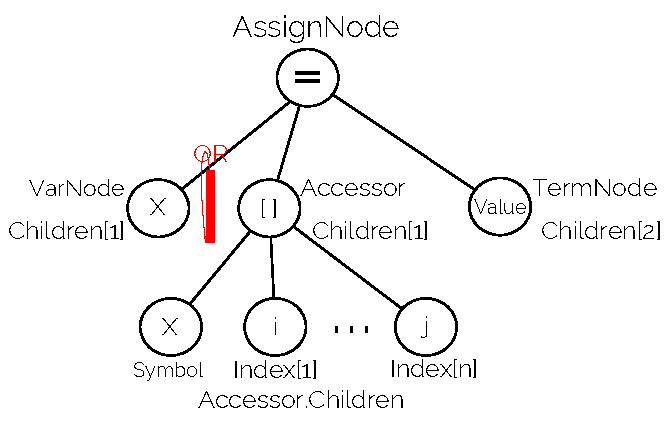
\includegraphics[width=0.6\textwidth]{images/assignnode.pdf}
\end{SCfigure}
Ahhoz, hogy megértsük az algoritmust, érdemes tisztázni, hogy hogyan néz ki gyakorlatban egy értékadó csúcs. A csúcs bal oldali gyereke szimbólum, vagy tömbhozzáférést kérő kifejezés. A jobb oldalán tetszőleges kifejezés állhat, aminek a Resolve (erről bővebben később) függvény segítségével először fel kell oldanunk az értékét az adott kontextusban. \\

% ábra a csúcsról?
Ha a bal oldalon csak egy szimbólum van, akkor egyszerűen odaadjuk a scope-nak a szimbólumot és a hozzá tartozó értéket tárolásra. \\
Ha tömbelem áll a bal oldalon, akkor az utolsó hozzáférést kérő indexig fel kell oldani Resolve-val a szimbólumok értékeit ( közben természetesen szemantikailag ellenőrizzük, hogy valóban tömbböt oldottunk fel ), majd értelemszerűen a feloldott tömb megfelelő indexén módosítjuk az értéket, és a teljes, eredeti tömböt a scope-nak adjuk tárolásra. \\
% optimalizálás?
\lstinputlisting[label=samplecode,caption=AssignNode bejárása]{sourcecode/walkassign}

%------------ Értékadáscsúcs bejárása

%------------ 

\subsubsection{Függvénycsúcs bejárása}
Függvényhívás utasításként nyilvánvalóan csak akkor szerepelhet, ha az adott függvénynek nincs visszatérési értéke. Bejárás szintjén ezeknek a csúcsoknak a feldolgozása igazából triviális, ugyanis az egyetlen feladat az, hogy a függvénycsúcs gyerekeit termekké feloldjuk Resolve segítségével, majd magán a függvényen az általa definiált CallFun metódust hívjuk. \\
Ez alól a szabály alól azonban kivételt képez a print függvény, mivel ennek implementációja speciális. Ennek részleteire későbbi fejezetben térek ki. 

\lstinputlisting[label=samplecode,caption=FunCallNode bejárása]{sourcecode/walkfuncall}

%------------ Függvénycsúcs bejárása

%----------------------------- Utasítások bejárása

\subsection{Kifejezések kiértékelése}

%----------------------------- 

%------------ 

\subsubsection{Aritmetikai csúcs kiértékelése}
Aritmetikai csúcsok bejárásához az AEGIScript definiál egy statikus NodeArithmetics nevű osztályt ( ennek az implementációjára szintén később térek ki ). Az eljárás lényege, hogy postfix gráfbejáráshoz hasonlóan meghatározzuk az adott szinten az aritmetikai kifejezés két argumentumát, majd átadjuk őket a NodeArithmetics-nek, ami már a megfelelő eredménnyel tér vissza.

\lstinputlisting[label=samplecode,caption=ArithmeticNode kiértékelése]{sourcecode/resolvearith}


%------------ Aritmetikai csúcs kiértékelése

%------------ 

\subsubsection{Függvény csúcs kiértékelése}
Lásd: \textit{2.5 algoritmus}. Az egyetlen különbség, hogy utolsó lépésben visszatérünk egy értékkel.

%------------ Függvény csúcs kiértékelése

%------------ 

\subsubsection{Tömbhozzáférés csúcs kiértékelése}
Lásd: \textit{2.6 algoritmus} tömbozzáférés csúcsra. Az egyetlen különbség, hogy utolsó lépésben nem Scope-hoz adjuk az értékét, hanem visszatérünk vele.

%------------ Tömbhozzáférés csúcs kiértékelése

%------------ 

\subsubsection{Tömbcsúcs kiértékelése}
Az AEGIScript dinamikusan típusos, így a tömbökben tetszőlegesen tárolhatunk akár különböző típusú értékeket is. Ennek megfelelően a tömbök kiértékelésére írt algoritmus végtelenül egyszerű: egyszerűen végigiterálunk a csúcs összes gyerekén, és kiértékelve hozzáadjuk ezek értékét az Elements mezőhöz, majd visszatérünk a tömbcsúccsal.

\lstinputlisting[label=samplecode,caption=ArrayNode kiértékelése]{sourcecode/resolvearray}

%------------ Tömbcsúcs kiértékelése

%------------ 

\subsubsection{Változócsúcs kiértékelése}
Változócsúcs esetén az egyetlen dolgunk delegálni az aktuális Scope-ot a VarNode által definiált Interpret eljárásnak, ami az adott kontextusban visszaadja a változó tényleges értékét
\lstinputlisting[label=samplecode,caption=VarNode kiértékelése]{sourcecode/resolvevar}



%------------ Változócsúcs kiértékelése


%------------ 

\subsubsection{Mezőhozzáférés csúcs kiértékelése}
Mezőhozzáférés esetén fontos megkötése a nyelvnek, hogy a hozzáférési lánc első elemének \textbf{kötelező} változószimbólumnak lennie, az összes többi helyen pedig csak függvényhívás állhat. Az algoritmus elsőként ezt a kezdőszimbúlumot kiértékeli, majd végigiterálunk a mezőhozzáférés csúcs összes elemén úgy, hogy ellenőrizzük hogy az iteráció előző eleme definiálja-e azt a függvényt, amit most próbálunk elérni. Ha igen, akkor kiértékeljük, majd erre folytatjuk ezt a láncot, amíg van elem.
\lstinputlisting[label=samplecode,caption=VarNode kiértékelése]{sourcecode/resolvefieldacc}


%------------ Mezőhozzáférés csúcs kiértékelése

%----------------------------- Kifejezések kiértékelése

%--------------------------------------------------- Absztrakt szintaxisfa bejárások
\newpage

\section{Technológiai háttér}

\subsection{C\# nyelv}

A C\# a Microsoft által fejlesztett modern, több paradigmát átölelő programozási nyelve. Első verzióját 2000-ben adták ki, azóta 4 nagy verzióváltáson esett át. Az ECMA sztenderd\cite{ecmacs} a következő elvárásokat állítja egy C\# implementáció elé: 

\begin{figure}[h!]
  \caption{\textit{A C\# nyelv fejlődése}}
  \centering
    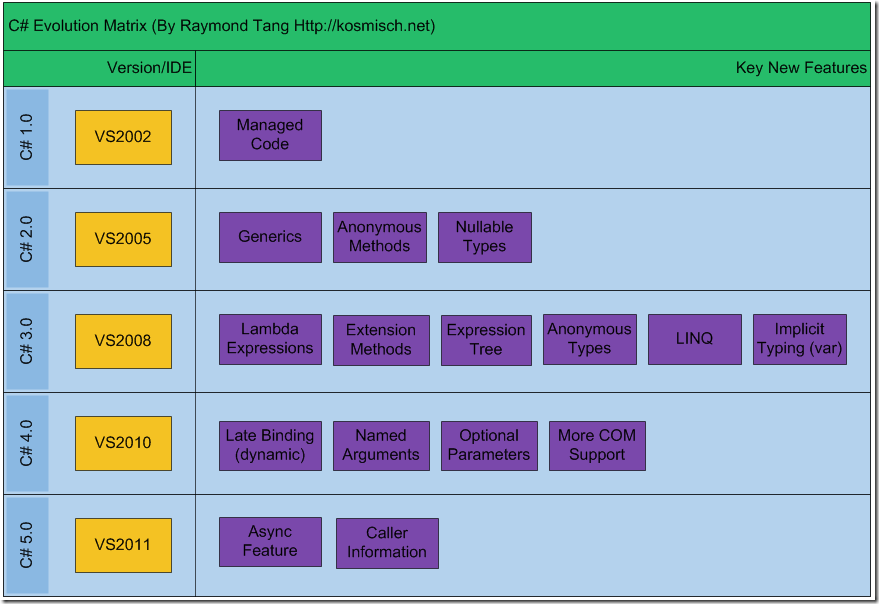
\includegraphics[width=0.9\textwidth]{images/csharpevolution.png}
\end{figure}

\begin{enumerate}

\item A C\# nyelv\cite{csharp} egy egyszerű, modern, általános célú, objektum-orientált nyelv.
\item A nyelvnek, illetve annak implementációinak biztosítania kell az erős típusosságot, tömb határ ellenőrzést, inicializálatlan változók használatának ellenőrzését és az automatikus szemétgyűjtést. A szoftverek robosztussága és a programozók produktivitása kiemelten fontos.
\item A nyelv célja, hogy szoftverkomponenseket fejlesszenek benne, amik kihelyezhetőek osztott rendszerekbe.
\item A forráskód érthetősége különösen fontos, főleg olyan programozók számára, akik eddig a C-t, C++-t vagy a Java-t ismerték.
\item A C\#-ban a célja, hogy minden méretű projekten és helyzetben jól működjön.
\item Bár a nyelvnek gazdaságosan kell bánnia a memóriával és processzoridővel, nem célja, hogy versenyre keljen a C-vel vagy Assemblyvel.

A C\# nyelv egyik legérdekesebb tulajdonsága az, hogy több programozási paradigmában is fejleszthetőek benne programok. Amióta bekerült a nyelvbe a LINQ (\textit{Language Integrated Native Query})\cite{linq} illetve a lambda kifejezések, nagyon könnyen lehet funkcionálisan programozni C\#-ban. \\

Az egyetlen rossz tulajdonság, ami felróható a C\# ellen, az az erős platform-függőség. Bár létezik implementációja a .NET keretrendszernek Linux-ra is Mono néven, ez távolról sem teljes, a később ismertetett Windows Presentation Foundation például csak Windows alapú rendszereken műmödik.

\end{enumerate}

%----------------------------- C# nyelv


\subsection{.NET keretrendszer}

A .NET keretrendszer\cite{dotnet} egy, a Microsoft által fejlesztett gyors alkalmazásfejlesztést segítő szoftverfejlesztői platform. A Sun Java platformjának közvetlen versenytársaként indította útjára a Microsoft 2002-ben. Azóta már a 4.5-ös verziónál jár a platform, és hatalmas a sikere Windowson. 

\subsubsection{A .NET felépítése}
A .NET alapját az CLI ( \textit{Common Language Infrastructure} ) képezi. Ez gyakorlatilag a leírása egy nyelvfüggetlen fejlesztői környezetnek, és ennek a környezetnek az implementációját .NET alatt CLR-nek ( \textit{Common Language Runtime} ) hívják. A CLR négy fő komponensből tevődik össze.

\begin{description}

    \item[Common Language Specification] A CLS a CLI része. Szabályokat ír le, amiket a kompatibilis nyelveknek be kell tartaniuk.
    \item[Common Type System] A CLI azon része, ami a típusokat, illetve azok egymással való interakcióit írja le. A .NET-ben implementált összes nyelv ugyanazt a típusrendszert használja, habár az elnevezésük lehet nyelvenként más és más.
    \item[Common Language Runtime] A .NET keretrendszer virtuális gépe. Itt kerül JIT fordításra a CIL bájtkód, amit az adott nyelv fordítója ad ki.
    \item[Common Intermediate Language] A CIL úgynevezett köztes kód, amire az összes CLI nyelvben írt program lefordul. Ezt a virtuális gép JIT fordítja natív kódra, amit már a processzor végre tud hajtani.


\end{description}

\begin{SCfigure}
  \caption{\textit{A .NET felépítése} \\ Látható, hogy a fordítás után már teljesen nyelvfüggetlen az egész keretrendszer.}
  \centering
    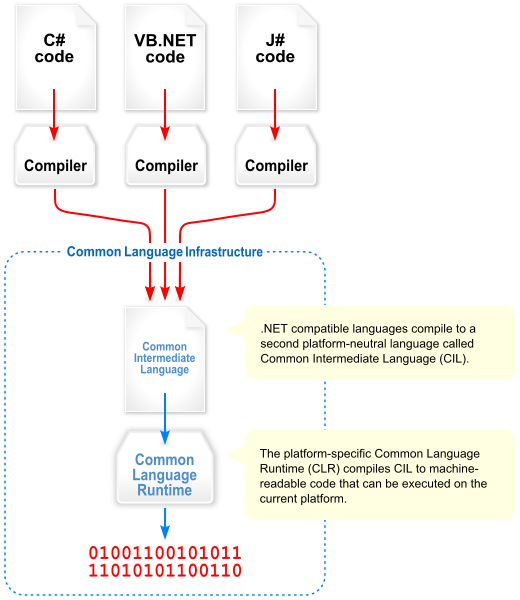
\includegraphics[width=0.6\textwidth]{images/dotnetinfrastructure.png}
\end{SCfigure}

A .NET rengeteg technológiát implementál, ami elősegíti a fejlesztői produktivitást. Ezek közül néhány:
\begin{description}
    \item[WinForms] Grafikus alkalmazások gyors fejlesztéséért felelő ablakkezelő rendszer.
    \item[ASP.NET] Dinamikus weboldalak létrehozására képes keretrendszer.
    \item[ADO.NET] Adatbázisok elérését megkönnyítő szolgáltatás.
    \item[WPF] Gazdag grafikus alkalmazások létrehozását segítő ablakkezelő rendszer. Bővebben később.
\end{description}

%----------------------------- NET keretrendszer


\subsection{Windows Presentation Foundation}

A WPF a Microsoft lépése egy modernebb ablakkezelő rendszer kiépítésére, a WinForms leváltására. Gyakorlatilag minden más ismert ablakkezelőtől eltérnek a WPF-ben megírt grafikus felületek, több okból is.

\subsubsection{XAML}
A WPF ablakok sémáját egy XML-hez hasonló, XAML (\textit{Extensible Application Markup Language}) nevű nyelvben kell leírni. Annak az oka, hogy egy grafikus felületet ilyen nyelven kelljen megfogalmazni, igen egyszerű és ésszerű: elválasztja a programozó és a grafikus felület tervezőjének munkáját. \\
A XAML szépsége abban rejlik, hogy amellett, hogy ablakok sémáját írhatjuk le benne, a felületen megjelenő különböző elemek formáját is megfogalmazhatjuk a segítségével. Kifejezetten UI dizájnereknek készült fejlesztői eszköz az Expression Blend, amivel kész XAML-alapú felületeket és stílusokat lehet tervezni a tényleges fejlesztői eszköztől, a Visual Studio-tól függetlenül.

\subsubsection{Az MVVM architektúra}
Az MVVM (\textit{Model-View-ViewModel})\cite{mvvm} architektúra a XAML mellett a másik ok, amiért sok fejlesztőt elrettent a WPF. A klasszikus Modell-Nézet architektúrához képest itt megjelenik egy új, nézetmodell nevű réteg is, ráadásul az architektúra tiltja, hogy a nézet akármikor közvetlenül elérje a modellt. \\
Az architektúra célja, hogy a lehető legjobban függetlenítse a kliens-oldali logikát a nézettől. A nézetnek és a modellnek a szerepe megegyezik a Modell-Nézet architektúrában lévővel, azonban szükség van egy harmadik rétegre, ami adatkötések, parancsok és absztrakciók révén állít hidat a két réteg között. \\
Az adatkötések ( \textit{Data Binding} ) kiemelt szerepet kapnak MVVM-ben. Egyszerűen arról van szó, hogy a nézet definiálhat akármelyik vezérlőjén, vagy akár az egész ablakon egy adatkontextust, ami egy nézetmodell lesz. Ezen nézetmodell publikus mezőit hozzáköthetjük a vezérlők bizonyos tulajdonságaihoz, amik változása tükröződni fog a nézeten.

\subsubsection{Egyéb szolgáltatások}
Az architekturális különbségek eleinte hátrányt jelentenek az MV architektúrából érkező fejlesztőknek, ám miután megismerik az MVVM-et és ki tudják aknázni a WPF által biztosított egyéb szolgáltatásokat, az áttérésbe fektetett energia többszörösen megtérül. A WPF egyéb szolgáltatásai:
\begin{description}
\item[Direct3D] A teljes ablakot képes a WPF Direct3D-n keresztül megjeleníteni, ami megengedi a Windowsnak, hogy a számítási költség egy részét a GPU-ra terhelje. Emellett lehetővé teszi az ablakokban a 3D renderelést is.
\item[Médiaszolgáltatások] A WPF rengeteg kép, zene és videoformátumot támogat.
\item[Animációk] A WPF segítségével könnyen lehet akár XAML-ben animációkat leírni.
\item[Szövegmegjelenítés] A WPF-ben különös hangsúlyt fektettek az igényes tipográfiára, aminek az oka egyértelművé vált a Windows 8 és a Metro-stílusú alkalmazások megjelenésével, amik ezt a szolgáltatást teljesen kiaknázzák.
\end{description}

%----------------------------- WPF

\subsection{Well-known text}

A Well-known text\cite{wkt} egy, vektorgeometriai objektumok térképes leírására szolgáló leíró nyelv. Bináris megfelelője a well-known binary, aminek a segítségével az olvasott adatokat közvetlenül tudjuk adatbázisokban tárolni. \\
Példa a Well-known text formátumra:

\begin{lstlisting}
GEOMETRYCOLLECTION(POINT(4 6),LINESTRING(4 6,7 10))
POINT ZM (1 1 5 60)
POINT M (1 1 80)
POINT EMPTY
MULTIPOLYGON EMPTY
\end{lstlisting}

%----------------------------- WKT


% link to ANTLR.org
\subsection{ANTLR v3.5}

Az ANTLR (\textit{ANother Tool for Language Recognition})\cite{antlr} egy nagyon fejlett parser-generátor eszköz, amit egy Terence Parr nevű egyetemi tanár fejleszt már két évtizede. Legfrissebb verziója a V4.0, ám ez egyelőre csak a Java targetet támogatja, az AEGIScript fejlesztése során én a v3.5-ös verzióra támaszkodtam. \\

Az ANTLR egy LL(*) parser-generátor, ami azt jelenti, hogy nem támogatja a bal rekurziót. Ezzel gyakran meggyűlik a baja azoknak, akik korábban Bisont használtak. Cserébe rengeteg zseniális funkcióval rendelkezik, mint például úgynevezett rewrite rule-ok, amiknek a segítségével a felismert szabályokat tetszőlegesen átírhatjuk más alakúra. \\

\begin{figure}[h]
  \caption{\textit{ANTLRWorks} \\ Az ANTLR által generált fa egy részfája az ANTLRWorks-ben egy AEGIScript forrásfájlról.}
  \centering
    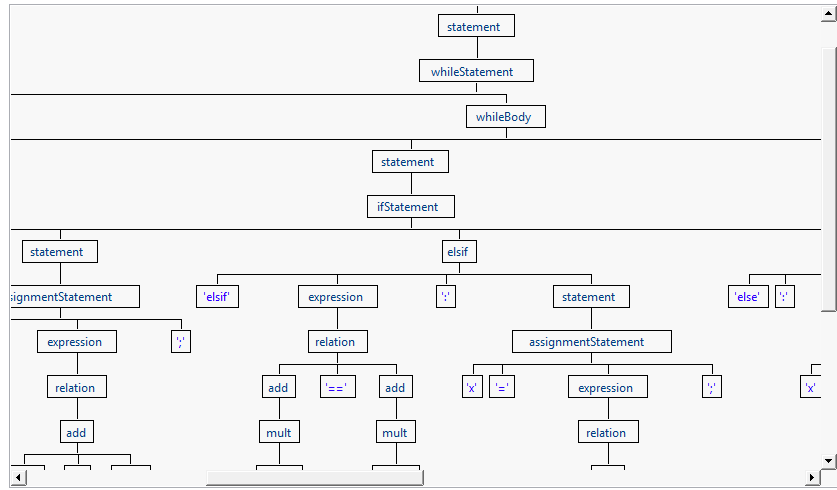
\includegraphics[width=0.8\textwidth]{images/parsetree.png}
\end{figure}

A legnagyobb pozitívuma az ANTLR-nek azonban a hihetetlenül fejlett fejlesztői környezete, amit ANTLRWorks-nek hívnak. Ebben lehetőség van a nyelvtanok lépésről-lépésre történő debuggolására, illetve képes grafikusan megjeleníteni a szabályok által létrehozott automatákat, vagy az adott forráskódból épített fákat. \\

Kimenete leggyakrabban egy absztrakt szintaxisfa, amelynek kezelésére azonban sajnos semmilyen segítséget sem nyújt a 3.5-ös verzió.

%----------------------------- ANTLR v3.5


%--------------------------------------------------- Technológiai háttér


% ------------------------------------------------------------------------------ Projektdefiníció



\chapter{Felhasználói dokumentáció}

\section{Rendszerkövetelmények}
A program telepítéséhez szükséges minimális rendszerkövetelményei a következők:
\begin{itemize}
    \item 1 GHz-es 32 bites (x86) processzor vagy 1 GHz-es 64 bites (x64) processzor
    \item 2 GB rendszermemória
    \item 8 MB szabad tárhely
    \item .NET 4.0 keretrendszer
    \item Windows Vista, vagy frissebb
\end{itemize}

Az ajánlott rendszerkövetelmények a következők:
\begin{itemize}
    \item 2 GHz-es processzor
    \item 4 GB rendszermemória
    \item 8 MB szabad tárhely
    \item Legalább 1366*768 felbontású monitor
    \item Windows 7, vagy frissebb
\end{itemize}

A program hardveres követelményei nagyban függenek attól, hogy milyen programokat írunk benne. Nagyméretű tömbök létrehozása során, vagy nagy ShapeFile-ok, Tiff-ek betöltése esetén számolni kell azzal, hogy megfelően több memóriát fog fogyasztani a program. \\

\section{A program telepítése}

Amennyiben a .NET keretrendszer már telepítve van, az AEGIScript telepítése nagyon könnyű. Egyszerűen le kell töltenünk egy .zip állományt, és ezt kicsomagolni egy tetszőleges helyre. Ezután a kicsomagolt mappában csak el kell indítani az AEGIScript.exe nevű futtatható állományt.


\section{A program használata}
\subsection{Kezdőképernyő}
\begin{figure}[h]
  \caption{\textit{Új ablak}}
  \centering
    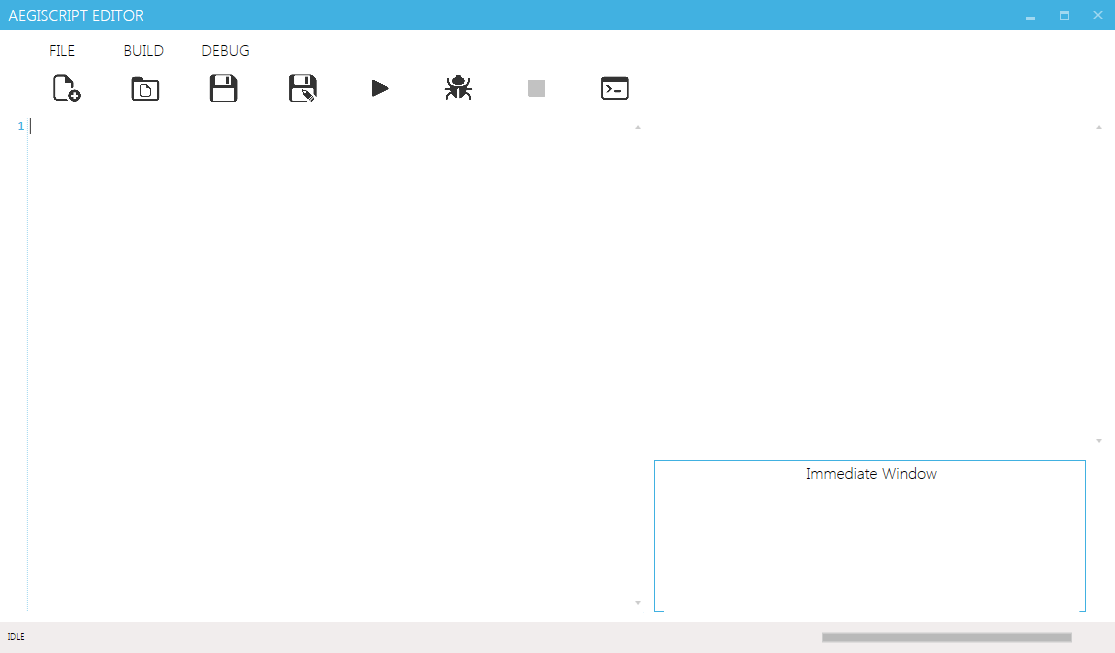
\includegraphics[width=0.85\textwidth]{images/newwindow.png}
\end{figure}
A program indítása után a fenti ábrán található látvány fogad minket. Alapértelmezetten az ablak 600x800-as méretben jelenik meg, ezt természetesen akármikor átméretezhetjük, de a kezdőméretnél kisebb szövegszerkesztésre nem optimális. \\
A felület java részét a bal oldali szövegszerkesztő, illetve a jobb oldali kimeneti ablak és az alatta található, úgynevezett 'immediate' ablak teszik ki. \\

\subsubsection{A menüsáv}
A program szolgáltat egy menüsávot, amin keresztül el tudunk érni minden olyan funkciót, amit egy szövegszerkesztőtől várunk. A menüsáv elemei: \\
\paragraph{File menü}
\begin{description}
\item[New file] Ezt az opciót választva a program eldobja a szövegszerkesztőben található jelenlegi szöveget, és új szövegszerkesztési munkamenetet indít.
\item[Open file] AEGIScript forrásfájl megnyitása a fájlrendszerből.
\item[Save file] A 'Save file' opció, amennyiben a fájlt korábban mentettük már, vagy a fájlrendszerből töltöttük be, a hely megkérdezése nélkül el fogja menteni a módosításokat, amiket a fájlon végeztünk. Amennyiben nem történt még mentés, a 'Save file as...' opció fog elindulni.
\item[Save file as] A jelenlegi szövegszerkesztési munkafolyamatot tudjuk elmenteni ezzel az opcióval a fájlrendszer egy tetszőleges helyére.
\item[Exit] Kilépés a programból.
\end{description}

\paragraph{Build menü}
\begin{description}
\item[Run] A szövegszerkesztőben lévő program futtatása normál módban. A kimenet a jobb oldali oszlopban jelenik meg.
\end{description} 

\paragraph{Debug menü - haladóknak} 
\begin{description}
\item[Print AST] Pretty printeli a kimeneti ablakba a szövegszerkesztőben lévő programból épített absztrakt szintaxisfát úgy, hogy a csúcsok ToString() metódusát hívja.
\item[Print AST Tokens] Pretty printeli a kimeneti ablakba a szövegszerkesztőben lévő programból épített absztrakt szintaxisfán található token típusokat és az azokhoz tartozó token értékeket.
\item[Print AST Objects] Pretty printeli nyersen az absztrakt szintaxisfán található objektumokat.
\end{description}

\newpage % később ellenőrizni!

\subsubsection{Az eszköztár}

A menüsávon kívül a program szolgáltat még egy sornyi gombot is vezérlésre, lásd az alábbi ábrán. A gombok sorrendben a következő funkcionalitást adják:
\begin{enumerate}
\item Új fájl
\item Fájl megnyitása
\item Fájl mentése
\item Fájl mentése mint
\item Futtatás
\item Futtatás a futási idejű hibák figyelmenkívül hagyásával
\item A futtatás megállítása
\item Az 'immediate' ablak tartalmának futtatása
\end{enumerate}
\begin{figure}[h]
  \caption{\textit{Az eszköztár}}
  \centering
    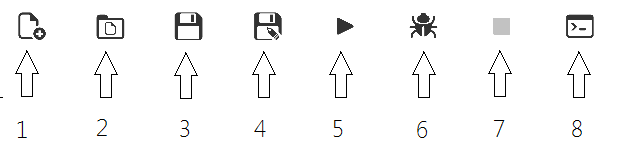
\includegraphics[width=0.8\textwidth]{images/gombok.png}
\end{figure}

\subsection{A nyelv használata}
Az AEGIScript által definiált nyelvet próbáltam a lehető legegyszerűbbé tenni, illetve minél hasonlóbbá az igen népszerű programozási nyelvhez, a Python-hoz. \\
Minden AEGIScriptben íródott programot a \textbf{begin} kulcsszóval kezdünk, és egy \textbf{end;} kulcsszóval zárjuk. Ezen két kulcsszó között tetszőlegesen sok állítást írhatunk le. Állítás lehet:
\begin{itemize}
\item[-] Értékadás
\item[-] Elágazás
\item[-] While ciklus
\item[-] Függvényhívás
\end{itemize}
Természetesen elágazásokban illetve ciklusokban tetszőleges mélységig ágyazhatóak egymásba állítások. \\
Az állítások kifejezésekből épülnek fel. Ezek a kifejezések lehetnek változónevek, primitív típusok, aritmetikai kifejezések, függvényhívások, vagy mezőelérések. \\

\lstinputlisting[label=samplecode,caption=Az AEGIScript nyelvtana]{sourcecode/grammar}

Példakódok megtalálhatók a letöltött .zip állomány TestCode mappájában.

\subsection{A kódszerkesztő szolgáltatásai}
A program az AvalonEdit\cite{avalon} nevű szövegszerkesztőt használja szerkesztőként, ami biztosítja a következő funkciókat:
\begin{itemize}
\item[-] Visszalépés : CTLR+Z
\item[-] Előrelépés : CTLR+Y
\item[-] Kódkiegészítés : a '.' karakter beütésére
\item[-] Syntax highlighting
\end{itemize}

Ezen felül a program biztosít néhány kényelmi funkciót szövegszerkesztésre, mint a fájl automatikus mentése a CTRL+S billentyűkombinációval, vagy a nem mentett módosítások jelzése a szerkesztő bal felső sakrában.

\begin{SCfigure}
  \caption{\textit{Nem mentett változások} \\ A bal felső sarokban található kis négyzet kéken világít, ha a jelenlegi munkamenetben még nem mentett változás található}
  \centering
    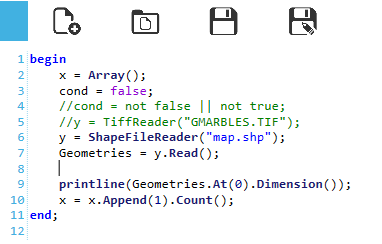
\includegraphics[width=0.5\textwidth]{images/filechanged.png}
\end{SCfigure}

A program által befiniált billentyűkombinációk:
\begin{description}
\item[Ctrl+N] Új fájl létrehozása, a szerkesztőben levő eldobásával.
\item[Ctrl+S] Jelenlegi fájl mentése. Amennyiben a fájl még nem került mentésre, egy felugró ablakban adhatjuk meg a helyét.
\item[Ctrl+O] Fájl megnyitása a fájlrendszerből.
\item[F4] A forráskód futtatása a futási idejű hibák figyelmen kívül hagyásával.
\item[F5] A forráskód futtatása.
\item[F6] A forráskódból épített absztrakt szintaxisfa tokenjeinek pretty printelése.
\item[F7] A forráskódból épített absztrakt szintaxisfa leveleinek objektum-szintű pretty printelése.
\end{description}

\subsection{A kimeneti ablak}
A kimeneti ablak a szerkesztőhöz hasonlóan szintén AvalonEditet\cite{avalon} használ, azonban a felhasználó nem tud írni bele. Ebben az ablakban jelennek meg a futtatott forráskód hibaüzenetei, eredményei, illetve a futtatás sikerességét és idejét jelző üzenet. \\
Mivel erre az ablakra tekintünk úgy, mint sztenderd kimenet, ezért a nyelv definiál egy print(), illetve egy printline() eljárást, amik segítségével a futás során akármikor kiirathatjuk változók, vagy kifejezések értékeit.

\subsection{Az immediate ablak}
Az immediate ablak azt a célt szolgálja, hogy egy program futtatása után, annak újrafuttatása, vagy módosítása nélkül, el tudjuk érni és tudjuk módosítani a program eredményét. \\
Ehhez elég beírnunk egy utasítást, vagy utasítások sorozatát begin és end kulcsszavak nélkül, majd meg kell nyomni az eszköztáron található 'Run immediate content' feliratú gombot. Ezután megtörténik az ablak tartalmának kiértékelése és kiírása a kimeneti ablakba. \\
Az immediate window definiál egy különleges parancsot, clear néven. Ha az ablak egyetlen bemenete a clear, vagy clear(), akkor a program kiüríti a kimeneti ablak, illetve az immediate ablak tartalmát.

\subsection{Az AEGIScript sztenderd könyvtára}
A következőkben az AEGIScript által definiált függvények következnek. Vastagon jelzem a függvény nevét, illetve közvetlenül mellette a függvény aritását.

\subsubsection{Speciális függvényutasítások}
\begin{description}
\item[print/1] Aszinkron kiírjuk a kimeneti ablakba a paraméter értékét string formájában. A fogadott paraméter akármilyen objektum, vagy kifejezés lehet.
\item[printline/1] Aszinkron kiírjuk a kimeneti ablakba a paraméter értékét string formájában sorvége karakterrel zárva. A fogadott paraméter akármilyen objektum, vagy kifejezés lehet.
\end{description}

\subsubsection{Speciális függvénykifejezések}
\begin{description}
\item[len/1] Visszaadja a kapott paraméter hosszát egész szám formájában. A fogadott paraméter lehet string, vagy tömb objektum.
\item[append/2] Visszaadja az első paramétert úgy, hogy hozzáfűzi a másodikat. Az első paraméter csak tömb lehet, a második akármilyen objektum.
\end{description}

\subsubsection{Tömbök függvényei}
\begin{description}
\item[Append/1] Hozzáfűzi a tömbhöz a paraméterül kapott értéket. A fogadott paraméter bármilyen típusú lehet.
\item[At/1] Visszatér a tömb paraméterül adott index helyén található értékkel. A fogadott paraméter egész szám.
\item[Count/0] Visszatér a tömb aktuális hosszával.
\item[RemoveAt/1] Kiveszi a tömbből a paraméterként kapott index helyén található értéket. A fogadott paraméter egész szám.
\end{description}


% ------------------------------------------------------------------------------


\chapter{Fejlesztõi dokumentáció}

A szakdolgozatom célja egy domain specifikus szkriptnyelv megvalósítása volt, melynek célja, hogy az AEGIS keretrendszer főbb eljárásait könnyen elérhetővé tegye egy alternatív felületen keresztül. Fontos szempont volt, hogy a nyelv később könnyen bővíthető legyen új nyelvi elemekkel, beépített osztályokkal vagy eljárásokkal, így megoldást kellett találnom a C\# generikusainak rugalmatlanságából adódó problémákra.\\

Az osztály-hierarchia felépítése során tehát törekedtem arra, hogy a megírt kód ipari színvonalú legyen, ne legyenek benne szélső esetek, amik problémákat okozhatnak, illetve igyekeztem tervezési minták segítségével a lehető legpragmatikusabb megoldásokat felhasználni a problémák megoldására. Komoly hangsúlyt fektettem arra is, hogy az osztályaim publikus interfészei a lehető legmagasabb absztrakciós szinten működjenek, ezzel is segítve a kódom, illetve a nyelv később használatát, bővítését. \\

Természetesen mivel egy programozási nyelv esetében kiemelten fontos a magas hibatűrés, így a már említett szélső esetek elkerülése mellett, rengeteg időt fektettem a felhasználó által elkerülhetetlenül előidézett hibák megfelelő jelzésére. Leszámítva a szintaktikai és lexikai hibákat, amiket az ANTLR\cite{antlr} sajnos elnyel és csak a hibák számát adja meg, a szemantikus és futási idejű hibákat könnyen érthető, beszédes hibaüzeneteken keresztül juttatom el a felhasználóhoz.

\section{A fejlesztés menete}
\subsection{Fejlesztői környezetek}
A tervezés során elsőként mérlegelnem kellett, hogy pontosan milyen szintaxisú nyelvet szeretnék létrehozni. A minél könnyebb használat érdekében ezért úgy terveztem meg az AEGIScript nyelvtanát, hogy minél közelebb legyen a pszeudokódhoz, illetve a Pythonhoz, de elkerülve utóbbinak indentálás alapú blokkjait. \\

Ezután ki kellett választanom a fejlesztőeszközöket, amiket a nyelv, illetve annak értelmezése során felhasználtam. A parser felépítésére az Irony.NET és az ANTLR közül a választás végül az utóbbira esett, főleg annál az oknál fogva, hogy lényegesen jobban dokumentált. ANTLR fejlesztéshez az Eclipse\cite{eclipse}  ANTLR IDE\cite{antlride} nevű pluginjét használtam, ami a már korábban említett ANTLRWorks szolgáltatásait integrálta bele az Eclipse-be. C\# fejlesztésére a választás a Visual Studio 2012-re esett.

\subsection{A nyelv megépítése}
A fejlesztés első szakasza a korábban megtervezett nyelv implementálása volt ANTLR alatt. Mivel konkrét elképzeléseim voltak a szintaxisról, így ezt a fázist gyorsan le tudtam zárni. Komolyabb kihívás a bal rekurzió kikerülése volt, illetve az AST újraírási szabályok megfelelő használata. Ezután, mivel az ANTLR C\# target-ének kimenete CommonTree típusú absztrakt szintaxisfák esetén nem túl részletes, így a következő lépés ennek megismerése volt, illetve az ilyen fák megjelenítésére egy megfelelő rendszer és grafikus felület felépítése.

\subsection{A grafikus felület tervezése}
A grafikus felület implementálására adott volt a Windows Presentation Foundation. Azonban mint kiderült, a WPF beépített szövegszerkesztője, amellett, hogy semmilyen formában nem támogat szintaxis kiemelést, már viszonylag rövid szövegek esetén is hajlamos belassulni, így kénytelen voltam egy külső könyvtár szövegszerkesztő vezérlőjét felhasználni. Az egyetlen opció az AvalonEdit\cite{avalon} volt, amit többek között a MonoDevelop nevű Linuxos .NET fejlesztői környezet is felhasznál. \\
Ezután a lehető legintuitívabbá próbáltam formálni a grafikus felületet, ikonok és menüsáv felvételével, illetve a más szövegszerkesztőkből megszokott billentyűparancsok segítségével. Emellett, hogy minél modernebb legyen a kinézete, tartottam magam a Microsoft Metro-stílusának vezérelveihez, illetve felhasználtam a MahApps \cite{mahapps} nevű külső könyvtárat, ami Metro-stílusú vezérlőket szolgáltat.

\subsection{A nyelvből épített fák megismerése}
A fejlesztés korai szakaszának legkritikusabb pontja volt az absztrakt szintaxisfák ANTLR-es reprezentációjának megismerése. Több pretty printelő eljárást is definiáltam, köztük in order és mélységi bejárás alapúakat, amik képesek voltak a grafikus felületre formázva kiírni a forráskódból épített fákat. Ezen kimenet alapján át kellett szabnom többször is az ANTLR-ben már megépített nyelvet, és a nyelvi elemekhez tartozó újraíró szabályokat. 

\subsection{A szintaxisfák bejárása, nyelvi elemek implementációja}
A következő lépés a már megfelelően reprezentált szintaxisfák értelmezése volt C\#-ban. \\
Az első próbálkozásom egy bytecode interpreter felépítése volt a Reflection könyvtár segítségével. Azonban hamar rájöttem, hogy egy ilyen interpreter megépítése jelentősen túlmutat a szakdolgozat céljain, hiszen teljesen triviális struktúrákból épített IL-kód kibocsájtása is jelentős problémákat okozott, ráadásul az egyetlen forrás, amiből építkezni tudtam az Kevin Hazzard és Jason Bock Metaprogramming in .NET\cite{metaprog} nevű könyve volt. Ezt a megközelítést is kénytelen voltam elvetni, és áttérni egy klasszikus AST interpreter felépítésére. \\

Ehhez konstruálnom kellett egy rendszert, amivel értelmezni tudtam az ANTLR által uniform, CommonTree típusú fákból álló szerkezetet. A létrehozott osztályszerkezet képes volt arra, hogy egy paraméterül kapott CommonTree-ből rekurzívan felépítsen maga alá egy, már saját osztályokból álló fastruktúrát, amin minden szükséges információ rendelkezésre állt az értelmezéshez.\\
Szükség volt még ezen felül láthatósági szabályok definiálására, illetve a változók tárolásának megvalósítására. Utóbbival kapcsolatban fontos döntés volt, hogy dinamikus, vagy statikus típusrendszert definiáljon az AEGIScript. A választás a dinamikus típusrendszerre esett, mivel sokkal nagyobb rugalmasságot ad mind a nyelv fejlesztése, mind a később felhasználása során. \\
Miután minden adott volt a nyelv teljes értelmezéséhez, elkezdtem implementálni a tényleges interpretert, ami csúcsok típusának megfelelően tudta értelmezni az általam definiált fákat

\subsection{Az AEGIS támogatása}
Az alapvető nyelvi elemek kiépítése, tesztelése és optimalizálása után következhetett az AEGIS keretrendszer támogatásának implementációja. Ehhez ki kellett találnom egy rendszert, amivel viszonylagos könnyedséggel bővíthetőek a különböző AEGIScript által definiált típusok új eljárásokkal. Ezen rendszer segítségével már viszonylag könnyen lehetett az AEGIS által definiált típusokat és eljárásokat AEGIScript-es formára alakítani.

\subsection{Well-known text beolvasása}
A Well-known text formátum beolvasására és értelmezésére az AEGIS-ben definiált eljárásokat használtam fel.




% ------------------------------------------------------------------------------

% ------------------------------------------------------------------------------


\chapter{Összegzés}

A feladatom egy térinformatikai szkriptnyelv megvalósítása volt a lehető legáltalánosabb, legkönnyebben kiegészíthető formában. Úgy gondolom, hogy ezt maximálisan sikerült elérni, hiszen az általam felépített osztálystruktúra könnyen értelmezhető és akármikor triviálisan bővíthető az AEGIS-ben megjelenő új osztályokkal vagy eljárásokkal. \\
Bár sokat segített a kötelező kurzusokon megszerzett általános programozási szemlélet, a szakdolgozat hatékony megírásához rengete \\
Ezen felül büszke vagyok az AEGIScript teljesítményére, hiszen az általam megírt algoritmusok a lehető legoptimálisabbak, amit a Visual Studio profilere is kiválóan mutat, nincsenek teljesítménybeli bottleneck-et képező eljárások. \\
Felhívnám a figyelmet a nyelv futási idejű hibaüzeneteire is, ezek ugyanis lényegesen beszédesebbek, mint az átlagos programozási vagy szkriptnyelv által adott, néha rejtvényszerű hibák.
\\

Bár a dolgozat megvalósítása során a kitűzött célokat elértem, feljesztés során több további továbbfejlesztési ötletem is támadt:
\begin{itemize}
	\item Viszonylag könnyen megvalósítható lenne a függvények objektumként való tárolása, illetve ilyen módon a függvény-objektumok tetszőleges paraméterezése.
	\item Lehetőség saját osztályok és eljárások definiálására futási időben. Ennek a megvalósítását is viszonylag könnyűvé teszi az általam épített osztálystruktúra.
	\item Saját kódgenerátor írása a különböző típusok közötti relációk leírására, illetve az AEGIS által definiált típusok leképezésére AST csúccsá. Előbbire a fejlesztés korai szakaszában el is kezdtem írni egy IronPython scriptet, ami egy egyszerű leíró nyelvből elő tudta állítani az aritmetikai kifejezéseket a különböző típusok között.
\end{itemize}

Összességében kijelenthetem, hogy remek kihívást nyújtott az AEGIScript megvalósítása, rengeteget tanultam az interpreterekről és a programozási nyelvekről általánosságban. Ezen felül különösen izgalmas volt a lazán összekapcsolt osztálystruktúra felépítése, illetve a teljesen rekurzív fabejáró eljárások létrehozása is, különösen azért, mivel korábban a rekurzió átlátása gondokat okozott.
Továbbá a fejlesztés során értettem meg a domainspecifikus nyelvek igazi erejét és a tényleges okot, amiért egyre több cég és nagyobb projekt használja őket. Egy DSL használatával ugyan a natív kódhoz képest érezhetően visszaesik a teljesítmény, azonban ezen az áron egy új absztrakciós szintet adhat a projektnek.


% ------------------------------------------------------------------------------


% ------------------------------------------------------------------------------

\listoffigures

\begin{thebibliography}{9}
\bibitem{dsl} \url{http://en.wikipedia.org/wiki/Domain-specific_language}
\bibitem{lip} Terence Parr: Language Implementation Patterns, The Pragmatic Bookshelf, 2009, ISBN: 978-1-93435-645-6
\bibitem{csharp} \url{http://msdn.microsoft.com/en-us/library/kx37x362.aspx}
\bibitem{ecmacs} \url{http://www.ecma-international.org/publications/files/ECMA-ST/Ecma-334.pdf}
\bibitem{dotnet} \url{http://msdn.microsoft.com/en-us/vstudio/aa496123.aspx}
\bibitem{antlr} \url{http://www.antlr.org}
\bibitem{eclipse} \url{http://www.eclipse.org/}
\bibitem{avalon} \url{https://github.com/icsharpcode/SharpDevelop/wiki/AvalonEdit}
\bibitem{mahapps} \url{http://mahapps.com/MahApps.Metro/}
\bibitem{metaprog} Kevin Hazzard, Jason Bock: Metaprogramming in .NET, Manning, 2013, ISBN: 978-1-61729-026-8
\end{thebibliography}

\end{document}
